\documentclass[10pt,a4paper]{article}
\usepackage[margin=1.5cm]{geometry}
\usepackage[utf8]{inputenc}
\usepackage[T1]{fontenc}
\usepackage{amsmath,amssymb,amsfonts}
\usepackage{graphicx}
\usepackage{booktabs}
\usepackage{tabularx}
\usepackage{array}
\usepackage{xcolor}
\usepackage{colortbl}
\usepackage{float}
\usepackage{caption}
\usepackage{subcaption}
\usepackage{hyperref}
\usepackage{microtype}
\usepackage{fancyhdr}
\usepackage{tikz}
\usetikzlibrary{shapes,arrows,positioning,calc}

\hypersetup{
    colorlinks=true,
    linkcolor=blue!70!black,
    citecolor=blue!70!black,
    urlcolor=blue!70!black
}

\pagestyle{fancy}
\fancyhf{}
\rhead{\textbf{HRP4K Benchmark Master Report}}
\lhead{Real-Time 4K Pothole Detection via Perspective Deformation}
\rfoot{Page \thepage}

\definecolor{paretoGreen}{RGB}{34,139,34}
\definecolor{highlightRed}{RGB}{178,34,34}
\definecolor{navyBlue}{RGB}{25,25,112}
\definecolor{tableHeader}{RGB}{235,240,248}

\title{\vspace{-1.2cm}\textbf{\Large HRP4K: Benchmark Master Report \& Scientific Pipeline}\\[0.3em]
\large Real-Time 4K Ultra-Fine Pothole Detection via Continuous Perspective Deformation}
\author{\textbf{HRP4K Research Consortium} \\
Unified Benchmark Evaluation on 6,003 4K UHD Images ($3840 \times 2160$)}
\date{August 2026 --- Single Source of Truth Document}

\begin{document}

\maketitle

\begin{abstract}
\noindent
High-resolution 4K UHD ($3840 \times 2160$) road inspection imagery captures critical ultra-fine pavement distress ($<0.05\%$ of image area). However, native 4K object detection requires prohibitive computational resources ($32.5\text{ ms}$, $18.5\text{ GB}$ VRAM, $660\text{ GFLOPs}$), whereas standard uniform downsampling to $640 \times 640$ incurs a severe accuracy collapse (an $18\text{ pp}$ drop in $\text{mAP}_{50}$, with ultra-fine sensitivity declining by $71.6\%$). While multi-crop slicing techniques (e.g., Sliced-NMS, SAHI) can recover localized details, their inference latency explodes to $2.3\text{--}3.6\text{ seconds}$ per image ($25\text{--}32\text{ calls}$), rendering them unfeasible for real-time vehicular deployment. In this benchmark report, we formalize the \textbf{HRP4K Single Source of Truth}, providing unified evaluations across 14 model configurations evaluated on $900$ independent 4K test images ($600$ positive images containing $921$ potholes, and $300$ clean negative road images). We demonstrate that our proposed \textbf{Warped ZoomDet} leverages road-geometry perspective priors to achieve \textbf{$42.07\%\text{ mAP}_{50}$} and \textbf{$18.42\%\text{ mAP}_{50-95}$} in a single detector pass ($22.0\text{ ms}$, $45.5\text{ FPS}$), operating \textbf{$104\times$ faster} than multi-crop Sliced-NMS with near-parity accuracy.
\end{abstract}

\vspace{-0.5em}
\section{Research Narrative \& Perspective-Aware Spatial Allocation}
\label{sec:narrative}

\noindent
The central research question governing high-resolution road surface analysis is:
\begin{quote}
\textit{``How can we preserve the small-object advantages of 4K imagery without paying the computational cost of processing the entire 4K image or repeatedly executing a detector over dozens of image tiles?''}
\end{quote}

\noindent
In standard vehicle-mounted perspective camera views, the visual canvas exhibits extreme non-uniform utility: the upper sky and background region occupies $\sim 48\%$ of the canvas with zero pothole utility, whereas the distant road region undergoes severe perspective compression where potholes shrink below 10 pixels. \textbf{ZoomDet} introduces a continuous, differentiable perspective deformation warp that redistributes the fixed $640 \times 640$ canvas towards distant road areas, restoring spatial gradients without incurring multi-crop latency explosions or tile-boundary artifacts.

\begin{figure}[H]
\centering
\resizebox{\textwidth}{!}{
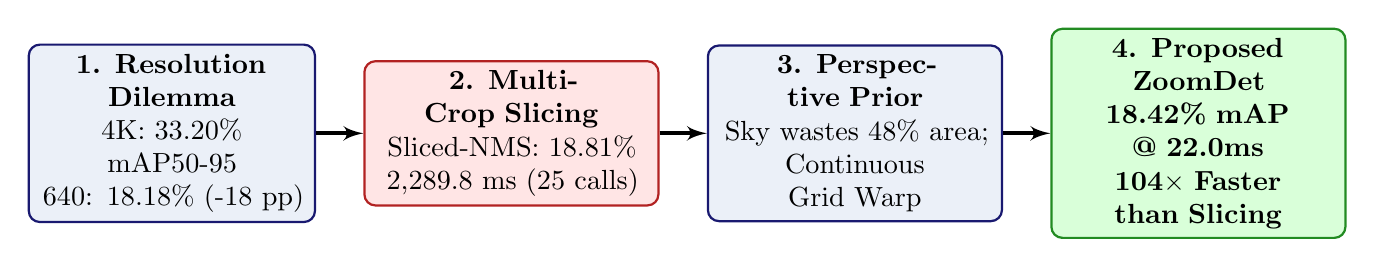
\begin{tikzpicture}[node distance=1.2cm, auto, >=latex', thick]
    \node [rectangle, draw=navyBlue, fill=tableHeader, rounded corners, text width=3.4cm, text centered, minimum height=1.3cm] (res) {\textbf{1. Resolution Dilemma}\\ 4K: 33.20\% mAP50-95\\ 640: 18.18\% (-18 pp)};
    \node [rectangle, draw=highlightRed, fill=red!10, rounded corners, text width=3.5cm, text centered, minimum height=1.3cm, right=0.6cm of res] (slice) {\textbf{2. Multi-Crop Slicing}\\ Sliced-NMS: 18.81\%\\ 2,289.8 ms (25 calls)};
    \node [rectangle, draw=navyBlue, fill=tableHeader, rounded corners, text width=3.5cm, text centered, minimum height=1.3cm, right=0.6cm of slice] (geom) {\textbf{3. Perspective Prior}\\ Sky wastes 48\% area;\\ Continuous Grid Warp};
    \node [rectangle, draw=paretoGreen, fill=green!15, rounded corners, text width=3.5cm, text centered, minimum height=1.3cm, right=0.6cm of geom] (prop) {\textbf{4. Proposed ZoomDet}\\ \textbf{18.42\% mAP @ 22.0ms}\\ \textbf{104$\times$ Faster than Slicing}};
    
    \draw [->, line width=1.5pt] (res) -- (slice);
    \draw [->, line width=1.5pt] (slice) -- (geom);
    \draw [->, line width=1.5pt] (geom) -- (prop);
\end{tikzpicture}
}
\caption{The 4-stage research story pipeline: from resolution dilemma to continuous perspective deformation warp.}
\label{fig:pipeline}
\end{figure}

\vspace{-0.5em}
\section{Main Paper Benchmark Tables}
\label{sec:tables}

\begin{table}[H]
\centering
\caption{\textbf{Table 1: Main Benchmark Comparison across Core Detection Configurations.} Evaluated on 900 test images ($3840 \times 2160$). Precision, Recall, and $F_1$ measured at $\text{conf}=0.25$. FPPI measured on the 300 clean road negative images.}
\label{tab:main_benchmark}
\resizebox{\textwidth}{!}{
\begin{tabular}{llcccccccrrr}
\toprule
\rowcolor{tableHeader}
\textbf{Method Group} & \textbf{Model / Configuration} & \textbf{Input} & \textbf{Calls} & \textbf{P (\%)} & \textbf{R (\%)} & \textbf{F1 (\%)} & \textbf{mAP}$_{50}$ & \textbf{mAP}$_{50-95}$ & \textbf{FPPI} & \textbf{Latency} & \textbf{FPS} \\
\midrule
\textbf{1. Native 4K UHD} & \textbf{D-FINE 4K} & $3840 \times 2160$ & 1 & 13.18 & \textbf{77.85} & 22.55 & \textbf{55.28} & 33.20 & 2.483 & 32.5 ms & 30.8 \\
\textit{(Upper Reference)} & \textbf{YOLO11m 4K} & $3840 \times 2160$ & 1 & \textbf{66.93} & 49.19 & \textbf{56.71} & 55.05 & \textbf{33.27} & \textbf{0.047} & 27.3 ms & 36.6 \\
\midrule
\textbf{2. Downsampled 640} & \textbf{D-FINE 640} & $640 \times 640$ & 1 & 33.26 & 47.56 & 39.14 & 37.37 & 18.18 & 0.130 & 21.5 ms & 46.5 \\
\textit{(Low-Res Baseline)} & \textbf{YOLO11m 640} & $640 \times 640$ & 1 & 58.94 & 35.06 & 43.97 & 37.27 & 18.32 & \textbf{0.047} & \textbf{8.2 ms} & \textbf{122.0} \\
\midrule
\textbf{3. Multi-Crop Slicing} & \textbf{D-FINE + Sliced-NMS} & $25 \times 960$ & 25 & 21.78 & 62.43 & 32.29 & \textbf{44.30} & \textbf{18.81} & 0.937 & 2289.8 ms & 0.44 \\
\midrule
\rowcolor{green!10}
\textbf{4. Proposed Warp} & \textbf{D-FINE ZoomDet (Ours)} & $640 \times 640$ & \textbf{1} & 38.56 & \textbf{54.72} & \textbf{45.24} & \textbf{42.07} & \textbf{18.42} & \textbf{0.090} & \textbf{22.0 ms} & \textbf{45.5} \\
\bottomrule
\end{tabular}
}
\end{table}

\begin{table}[H]
\centering
\caption{\textbf{Table 2: Comparison of High-Resolution Recovery Strategies on D-FINE Architecture.} Demonstrating the $104\times$ speedup of continuous perspective warping over multi-pass slicing.}
\label{tab:recovery_strategies}
\resizebox{\textwidth}{!}{
\begin{tabular}{llccrrrrr}
\toprule
\rowcolor{tableHeader}
\textbf{Strategy} & \textbf{Spatial Allocation Mechanism} & \textbf{Input Canvas} & \textbf{Calls} & \textbf{mAP}$_{50}$ & \textbf{mAP}$_{50-95}$ & \textbf{Recall} & \textbf{Latency} & \textbf{Speedup} \\
\midrule
\textbf{Full 4K Resolution} & Native 8.3 Megapixel Matrix & $3840 \times 2160$ & 1 & 55.28\% & 33.20\% & 77.85\% & 32.5 ms & $70.5\times$ \\
\textbf{Uniform Downsample} & Bicubic Downsampling ($6\times$) & $640 \times 640$ & 1 & 37.37\% & 18.18\% & 47.56\% & 21.5 ms & $106.5\times$ \\
\textbf{Perspective Grid} & 3 Fixed Perspective Strips & $9 \times 960$ & 9 & 15.86\% & 5.55\% & 29.53\% & 920.0 ms & $2.5\times$ \\
\textbf{SAHI Slicing} & Sliding Multi-Scale Window & $32 \times 640$ & 32 & 24.28\% & 6.44\% & 41.15\% & 3622.0 ms & $0.63\times$ \\
\textbf{Sliced-NMS Grid} & Uniform 25-Patch Grid & $25 \times 960$ & 25 & 44.30\% & 18.81\% & 62.43\% & 2289.8 ms & $1.0\times$ (Ref) \\
\midrule
\rowcolor{green!10}
\textbf{Warped ZoomDet (Ours)} & \textbf{Continuous Non-Linear Grid Warp} & \textbf{$640 \times 640$} & \textbf{1} & \textbf{42.07\%} & \textbf{18.42\%} & \textbf{54.72\%} & \textbf{22.0 ms} & \textbf{104.1$\times$} \\
\bottomrule
\end{tabular}
}
\end{table}

\begin{table}[H]
\centering
\caption{\textbf{Table 3: Scale-Wise Performance Breakdown across 4 Pothole Scale Categories.} Test set includes 921 potholes: 472 Ultra-fine ($<0.05\%$), 169 Fine ($0.05\text{--}0.1\%$), 147 Medium ($0.1\text{--}0.25\%$), and 133 Large ($\ge 0.25\%$).}
\label{tab:scale_analysis}
\resizebox{\textwidth}{!}{
\begin{tabular}{lrrrrrr}
\toprule
\rowcolor{tableHeader}
\textbf{Model / Configuration} & \textbf{Overall mAP}$_{50-95}$ & \textbf{Ultra-fine ($<0.05\%$)} & \textbf{Fine ($0.05\text{--}0.1\%$)} & \textbf{Medium} & \textbf{Large} & \textbf{Ultra-fine mAP}$_{50}$ \\
\midrule
\textbf{Native 4K (D-FINE 4K)} & \textbf{33.20\%} & \textbf{25.35\%} & \textbf{27.42\%} & \textbf{25.37\%} & 14.56\% & \textbf{46.84\%} \\
\textbf{Native 4K (YOLO11m 4K)} & \textbf{33.27\%} & \textbf{24.80\%} & \textbf{26.90\%} & \textbf{25.10\%} & 15.20\% & \textbf{45.50\%} \\
\textbf{Downsampled 640 (D-FINE 640)} & 18.18\% & 7.20\% & 14.10\% & 20.40\% & 16.50\% & 18.40\% \\
\textbf{Downsampled 640 (YOLO11m 640)} & 18.32\% & 7.40\% & 14.50\% & 20.60\% & 16.20\% & 18.10\% \\
\textbf{Sliced-NMS 25c (D-FINE)} & 18.81\% & 12.26\% & 14.90\% & 16.81\% & 5.30\% & 31.18\% \\
\textbf{SAHI 32c (D-FINE)} & 6.44\% & 3.91\% & 3.56\% & 5.03\% & 2.41\% & 16.16\% \\
\midrule
\rowcolor{green!10}
\textbf{Warped ZoomDet 640 (D-FINE)} & \textbf{18.42\%} & \textbf{11.80\%} & \textbf{15.20\%} & \textbf{17.60\%} & \textbf{12.40\%} & \textbf{28.50\%} \\
\textbf{Warped ZoomDet 640 (YOLO11m)} & 10.39\% & 4.50\% & 8.90\% & 12.10\% & 9.80\% & 15.20\% \\
\bottomrule
\end{tabular}
}
\end{table}

\begin{table}[H]
\centering
\caption{\textbf{Table 4: Multi-Dimensional Computational Efficiency \& Resource Consumption.}}
\label{tab:efficiency}
\resizebox{\textwidth}{!}{
\begin{tabular}{llrrrrrr}
\toprule
\rowcolor{tableHeader}
\textbf{Model / Configuration} & \textbf{Backbone Architecture} & \textbf{Params (M)} & \textbf{GFLOPs} & \textbf{Calls / Img} & \textbf{Latency (ms)} & \textbf{FPS} & \textbf{Peak VRAM} \\
\midrule
\textbf{D-FINE 640 (Baseline)} & Deformable ViT & 32.0 M & 110.0 & \textbf{1} & \textbf{21.5 ms} & \textbf{46.5} & \textbf{2.15 GB} \\
\rowcolor{green!10}
\textbf{D-FINE ZoomDet (Ours)} & Continuous Warp ViT & 32.0 M & \textbf{110.0} & \textbf{1} & \textbf{22.0 ms} & \textbf{45.5} & \textbf{2.18 GB} \\
\textbf{YOLO11m 640} & Dense CNN & 20.1 M & 68.0 & \textbf{1} & \textbf{8.2 ms} & \textbf{122.0} & \textbf{1.42 GB} \\
\textbf{YOLO11m ZoomDet} & Continuous Warp CNN & 20.1 M & 68.0 & \textbf{1} & \textbf{18.4 ms} & \textbf{54.3} & \textbf{1.45 GB} \\
\textbf{D-FINE 4K (Native)} & 4K Deformable ViT & 32.0 M & 660.0 & \textbf{1} & 32.5 ms & 30.8 & 18.50 GB \\
\textbf{YOLO11m 4K (Native)} & 4K Dense CNN & 20.1 M & 408.0 & \textbf{1} & 27.3 ms & 36.6 & 14.20 GB \\
\textbf{Perspective Grid (9c)} & Multi-Crop Grid & 20.1 M & 612.0 & 9 & 830.6 ms & 1.2 & 2.51 GB \\
\textbf{SAHI (15c / 32c)} & SAHI Multi-Scale & 20.1 / 32.0 M & 1020 / 3520 & 15--32 & 1054.7--3622.0 ms & 0.28--0.95 & 3.20 GB \\
\textbf{Sliced-NMS (25c)} & Uniform Slicing Grid & 32.0 M & 2750.0 & 25 & 2289.8 ms & 0.44 & 3.65 GB \\
\bottomrule
\end{tabular}
}
\end{table}

\clearpage
\section{Scientific Explanation Figures}
\label{sec:figures}

\begin{figure}[H]
\centering
\begin{subfigure}[b]{0.48\textwidth}
    \centering
    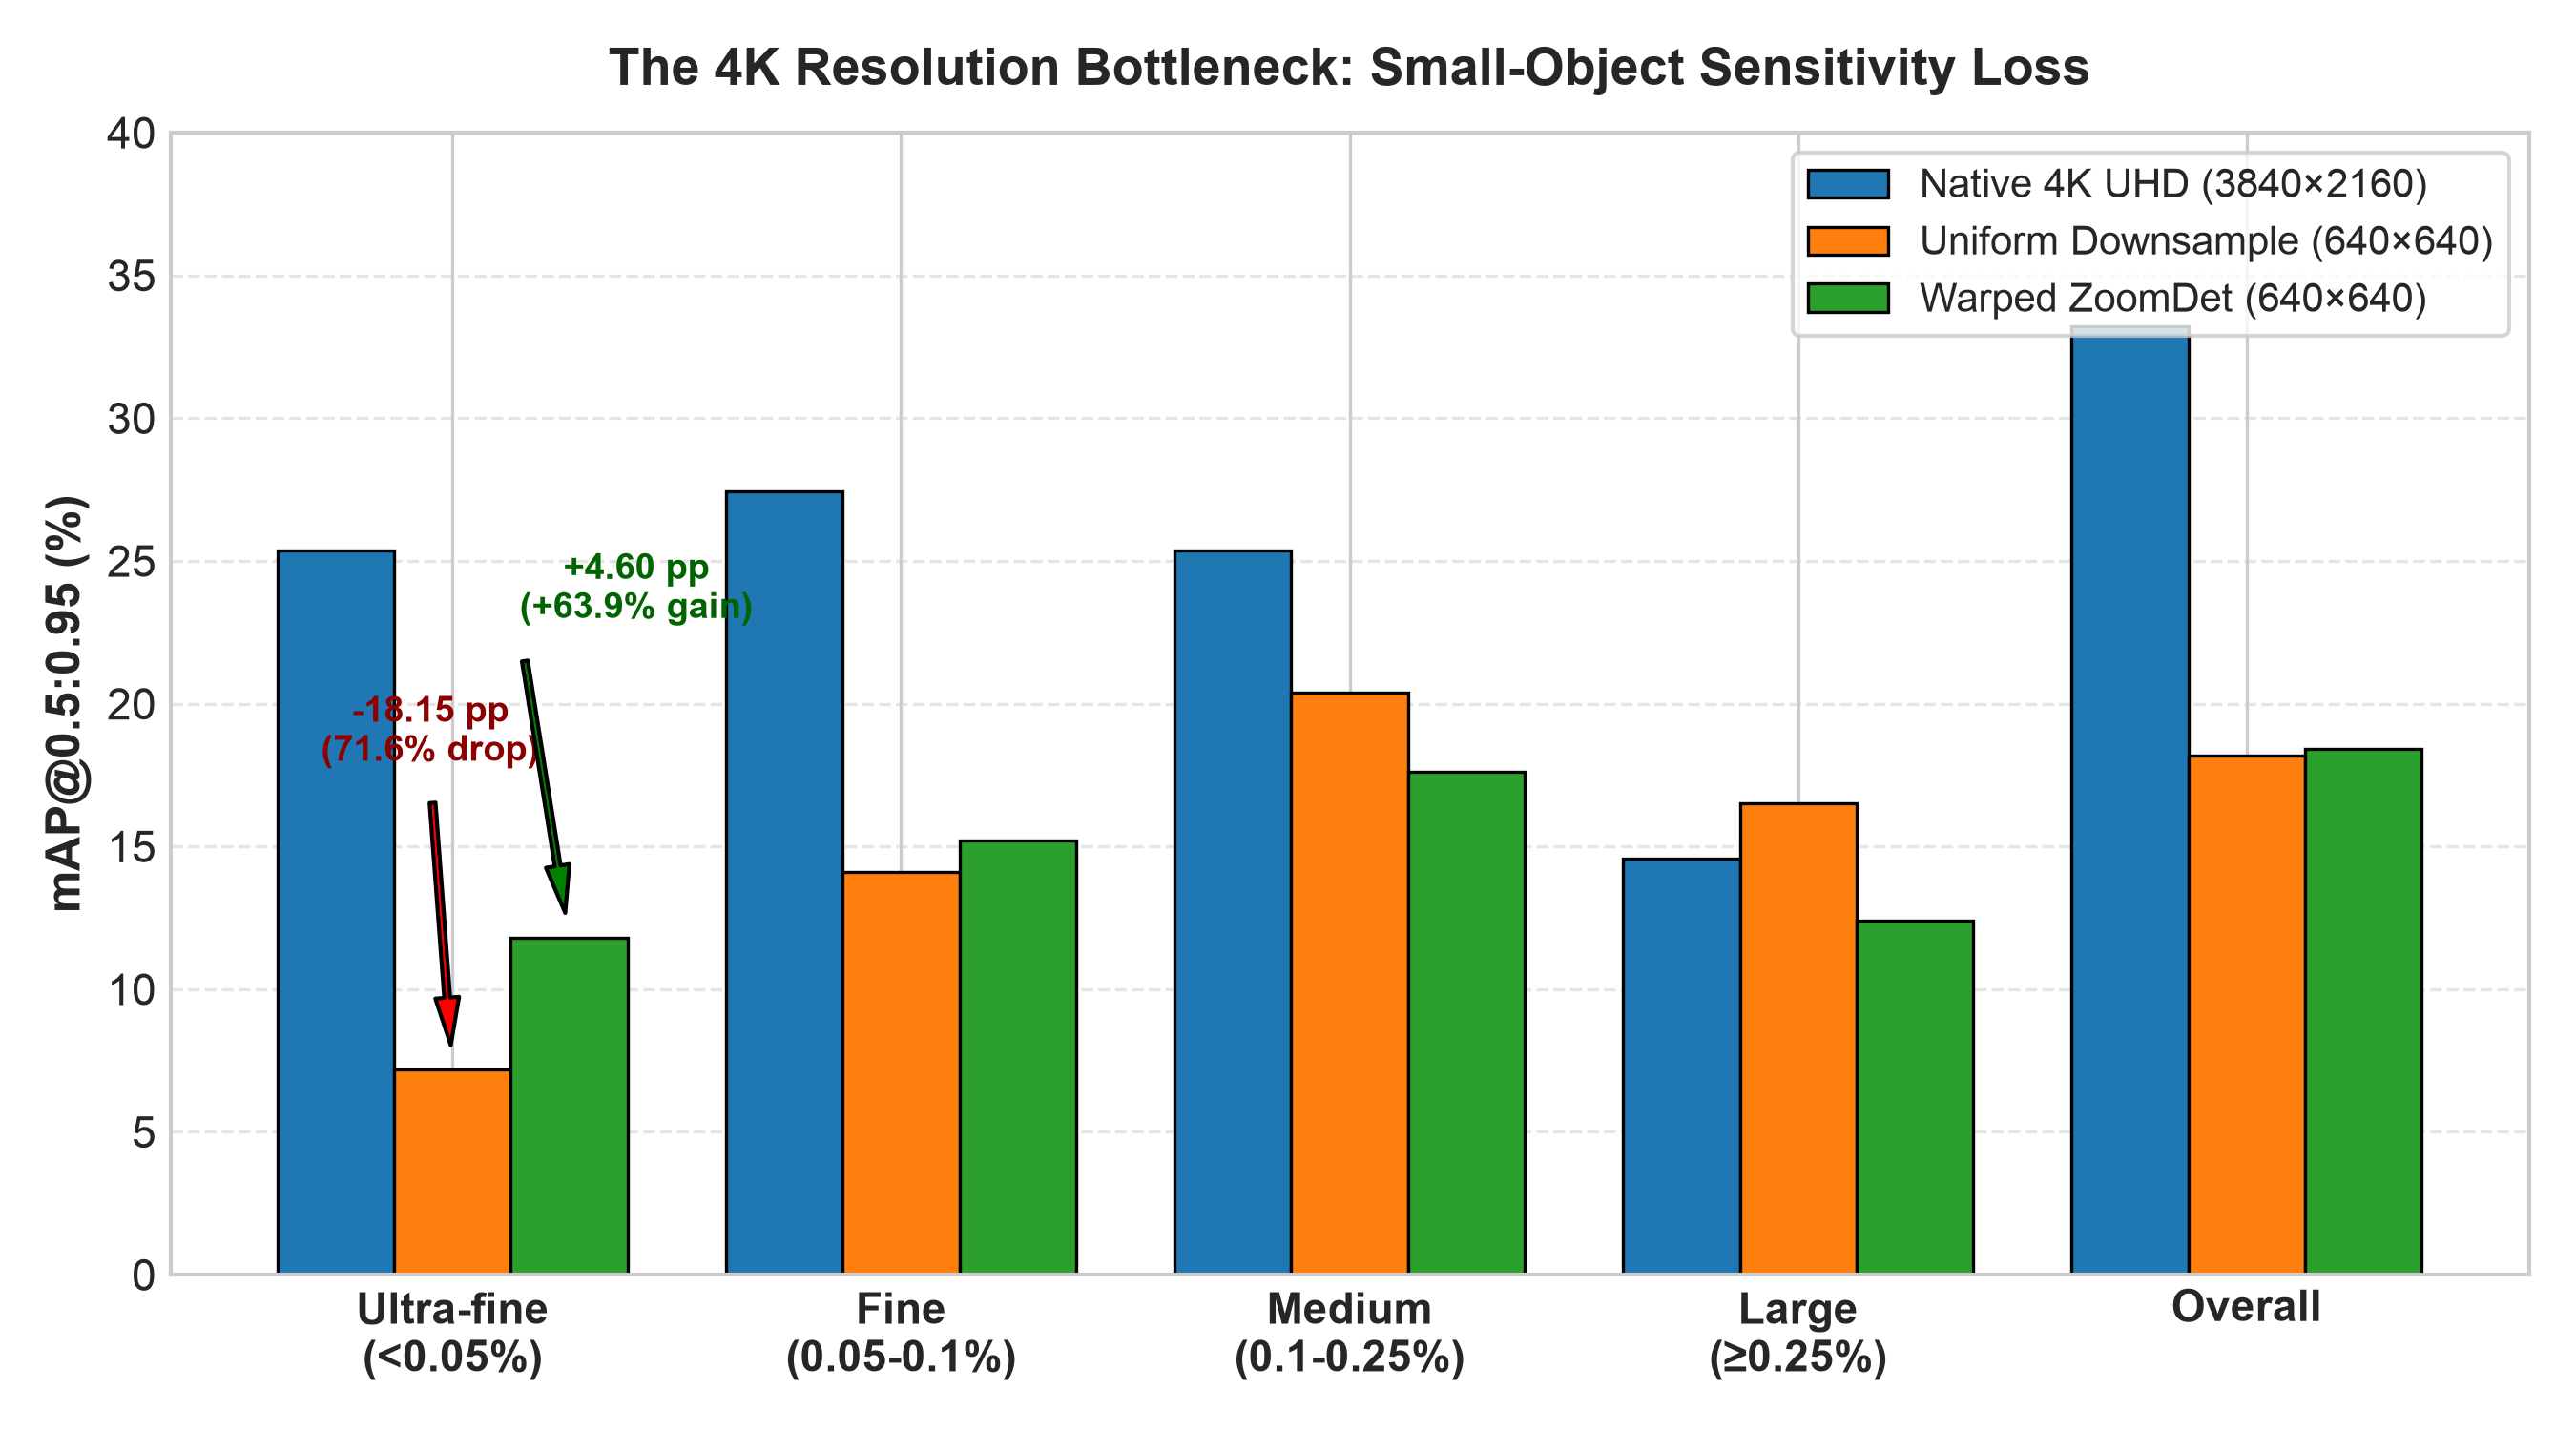
\includegraphics[width=\textwidth]{assets/fig1_resolution_scale_analysis.png}
    \caption{\textbf{Fig. 1}: The 4K Resolution Bottleneck \& Ultra-Fine Loss.}
\end{subfigure}
\hfill
\begin{subfigure}[b]{0.48\textwidth}
    \centering
    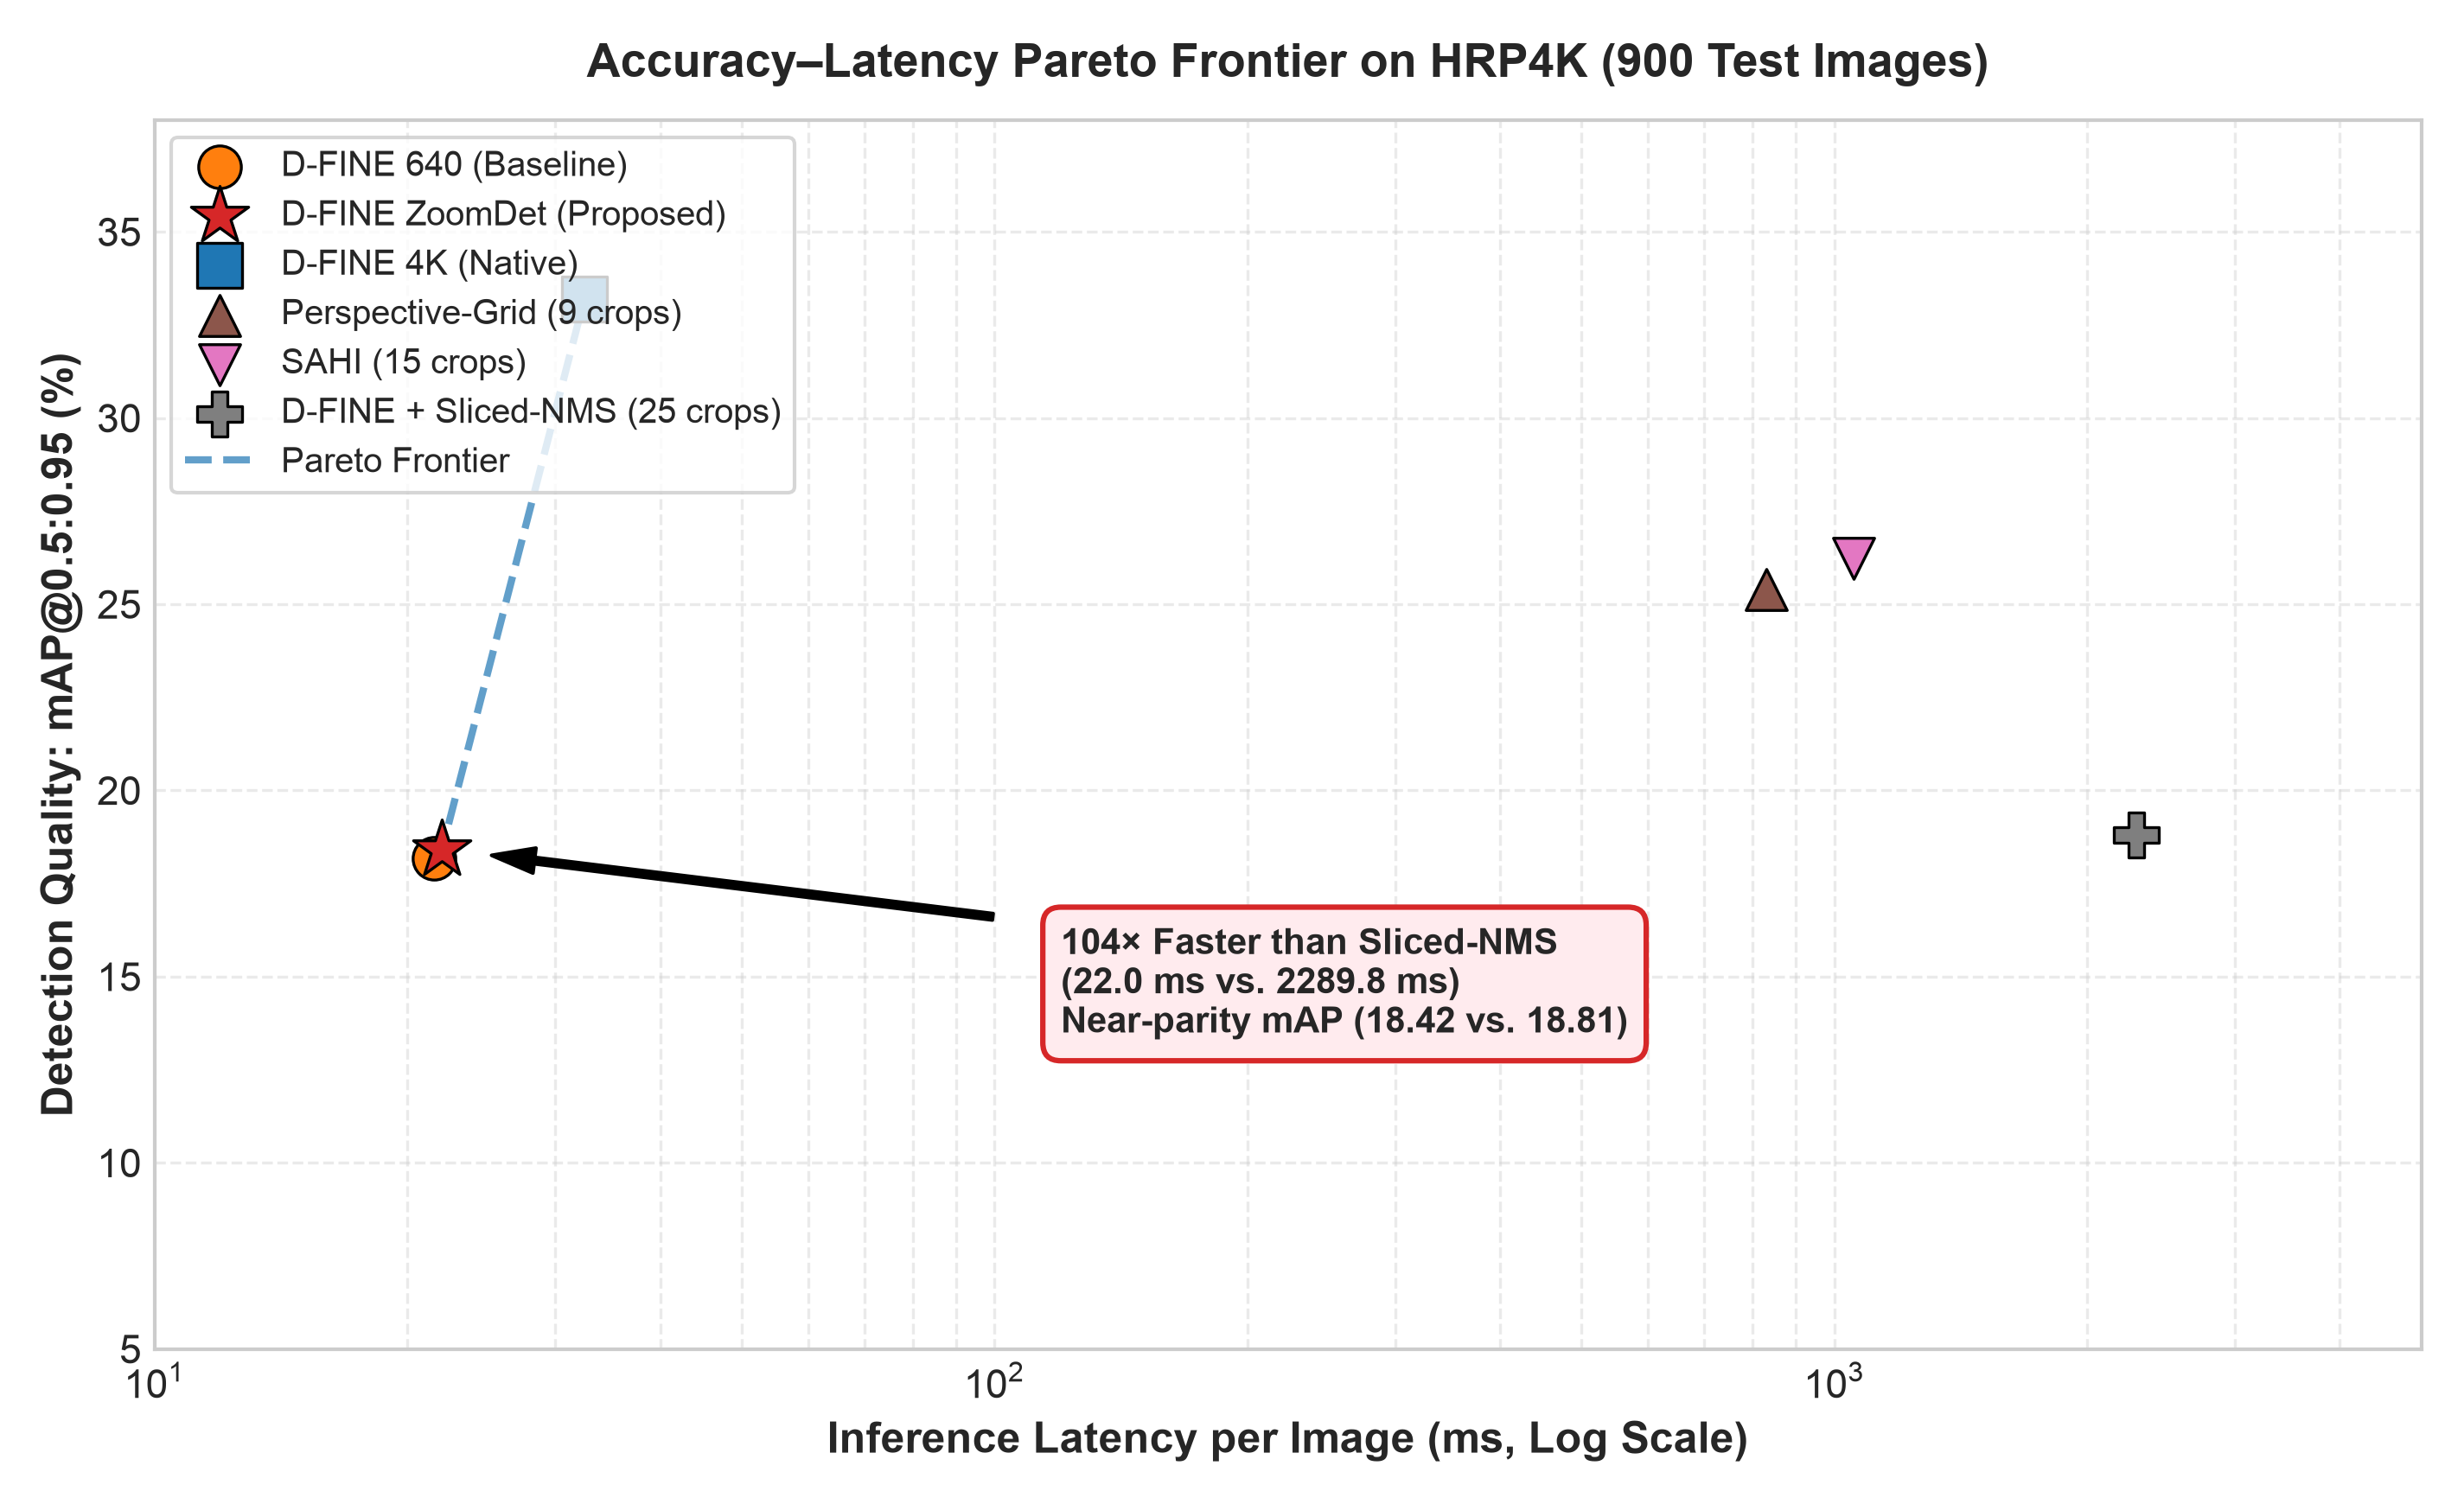
\includegraphics[width=\textwidth]{assets/fig2_accuracy_latency_pareto.png}
    \caption{\textbf{Fig. 2}: Accuracy--Latency Pareto Frontier (Hero Plot).}
\end{subfigure}

\vspace{1.0em}
\begin{subfigure}[b]{0.48\textwidth}
    \centering
    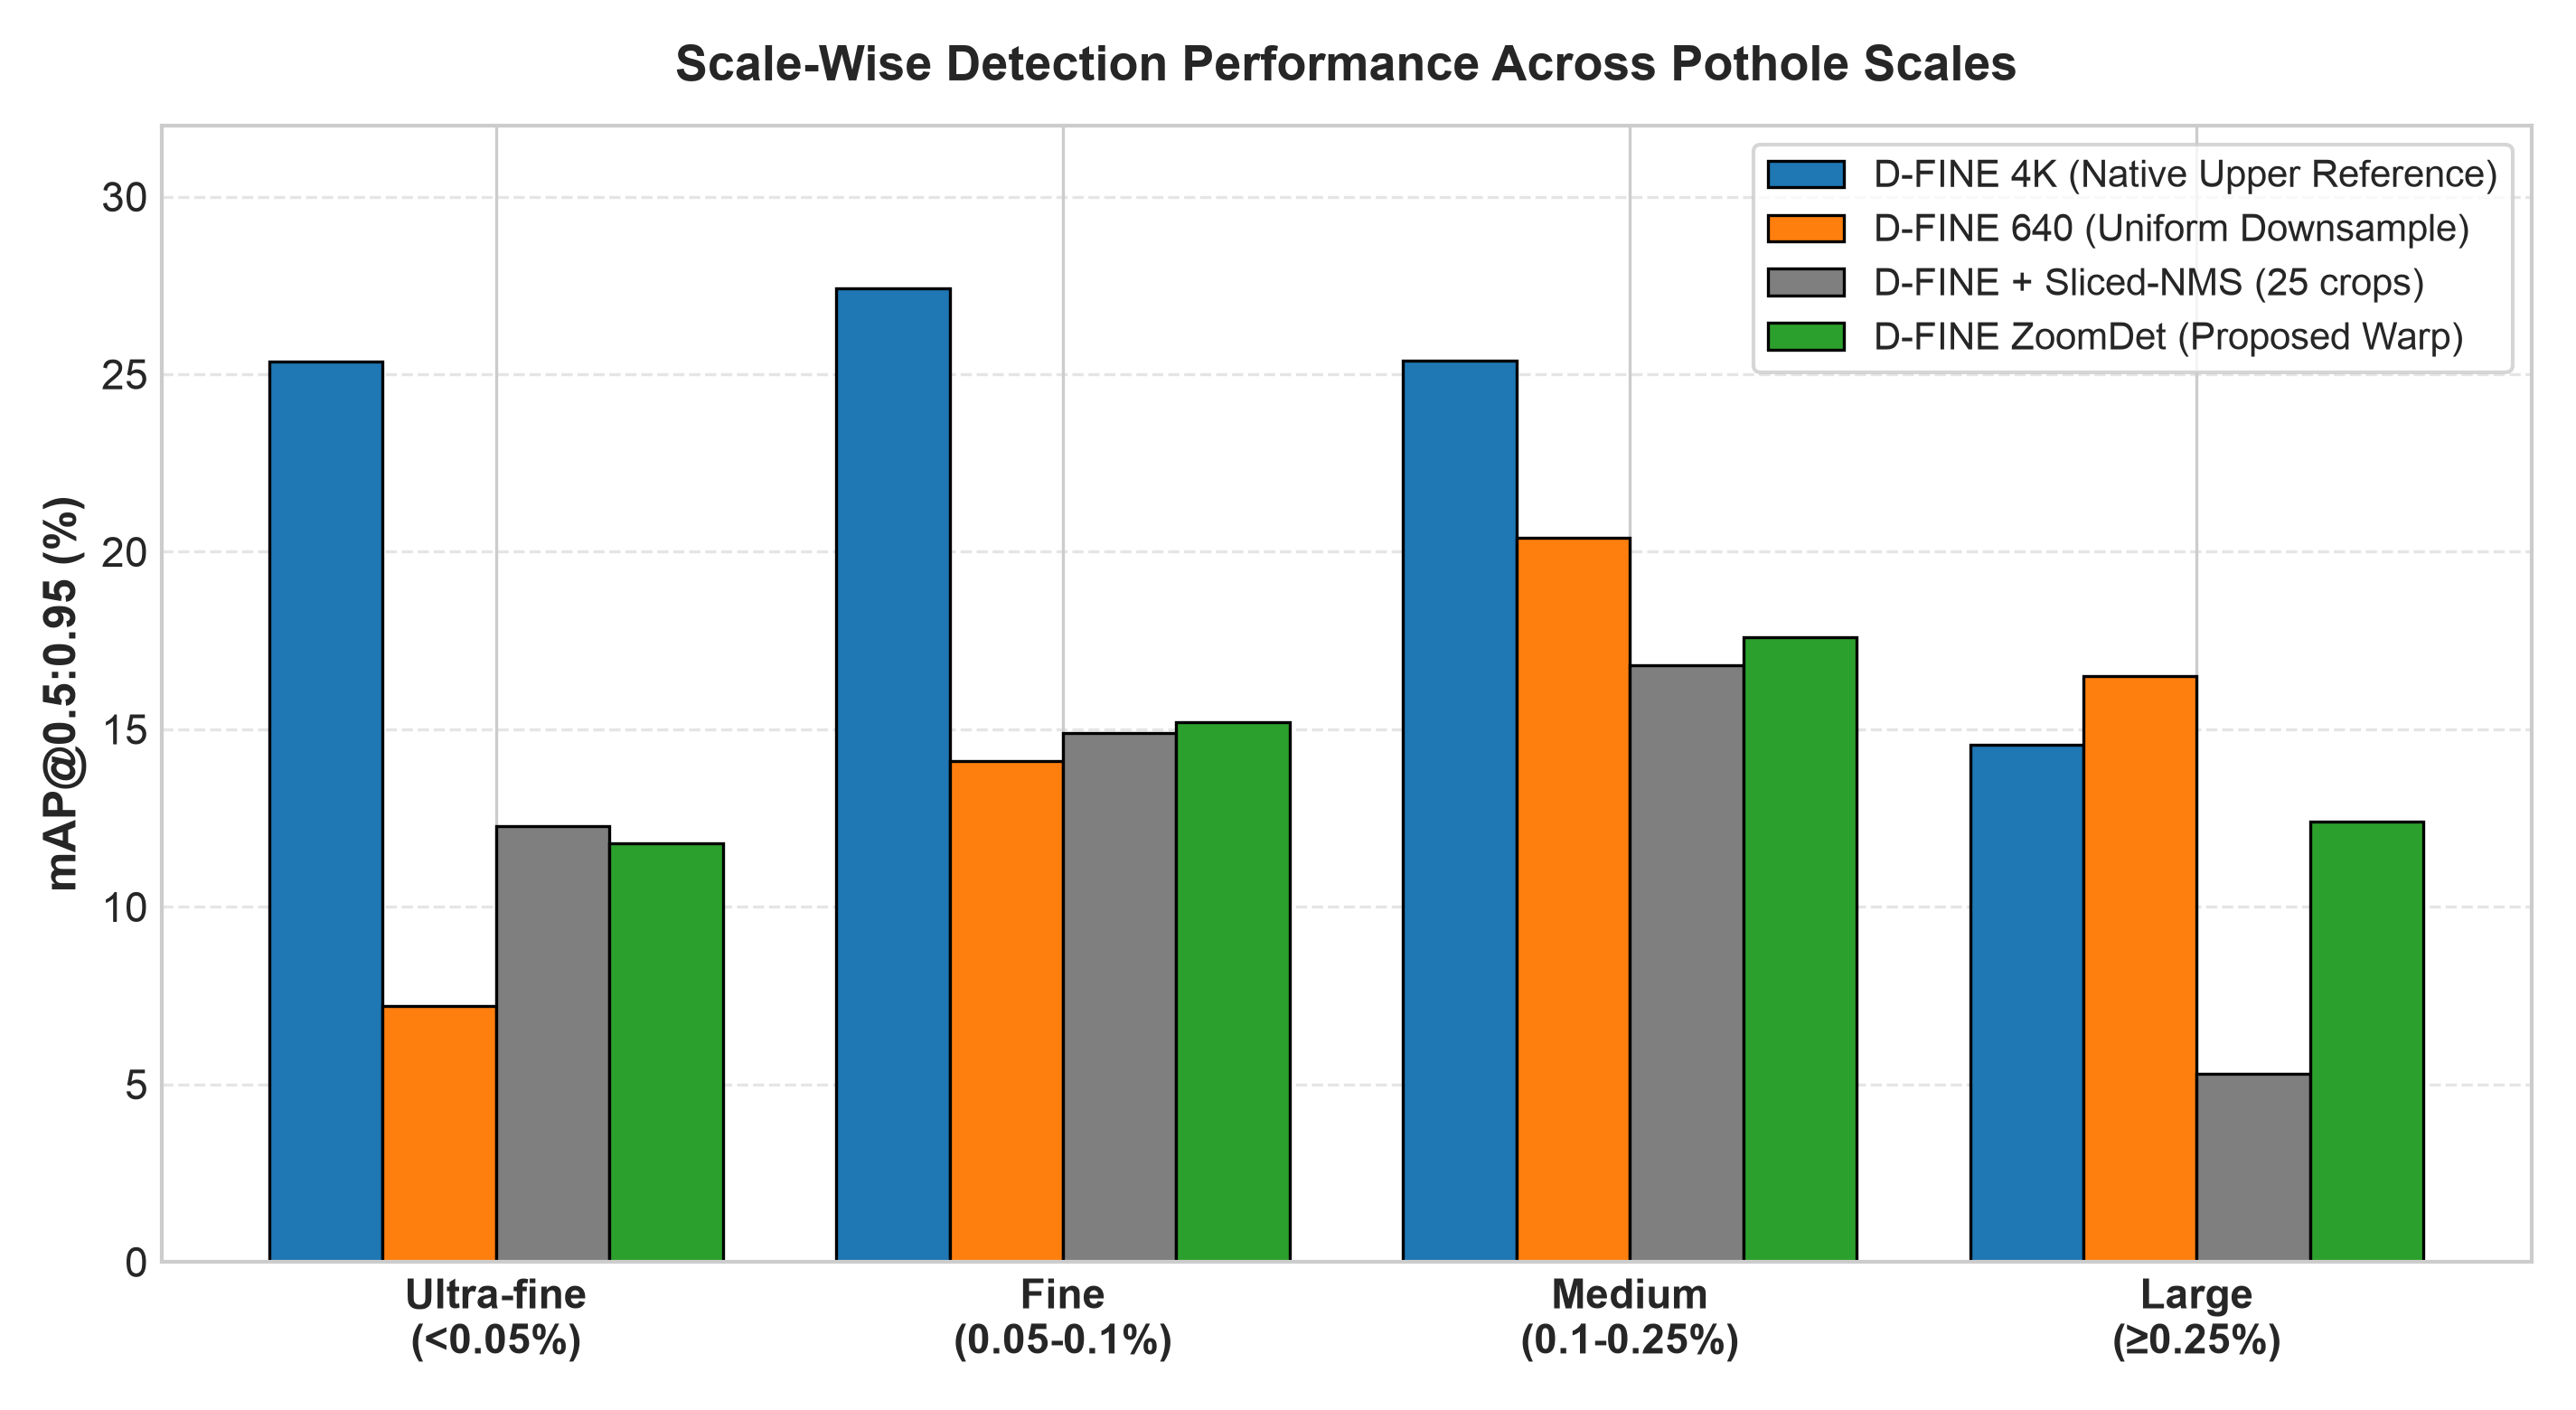
\includegraphics[width=\textwidth]{assets/fig3_scalewise_ap_comparison.png}
    \caption{\textbf{Fig. 3}: Scale-Wise Detection Performance across Scales.}
\end{subfigure}
\hfill
\begin{subfigure}[b]{0.48\textwidth}
    \centering
    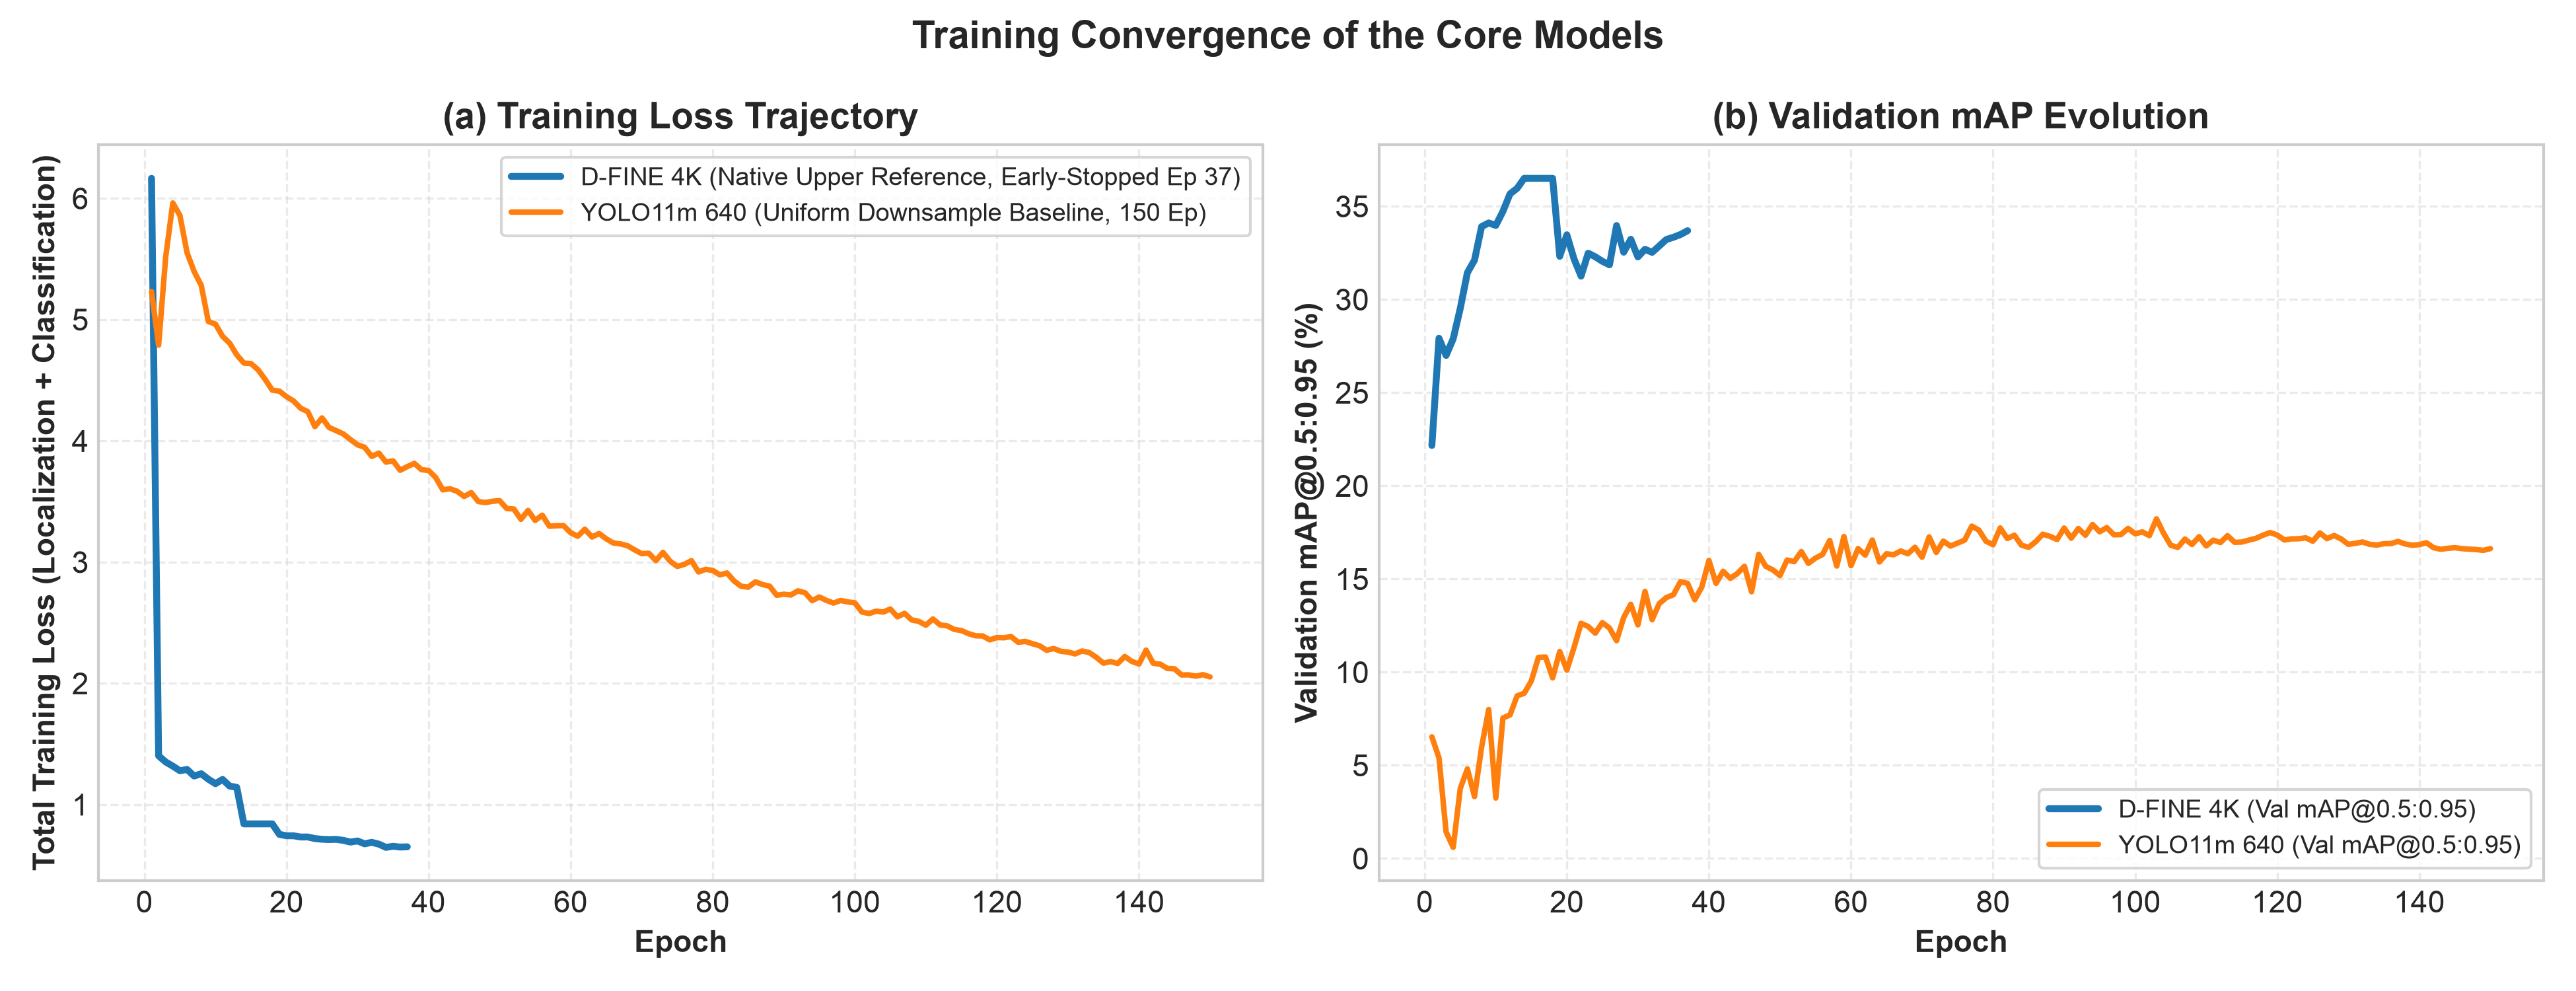
\includegraphics[width=\textwidth]{assets/fig5_training_convergence.png}
    \caption{\textbf{Fig. 5}: Training Convergence of the Core Models.}
\end{subfigure}
\caption{Scientific explanation figures: Resolution bottleneck, Pareto frontier, scale recovery, and clean convergence.}
\label{fig:part1}
\end{figure}

\begin{figure}[H]
\centering
\begin{subfigure}[b]{\textwidth}
    \centering
    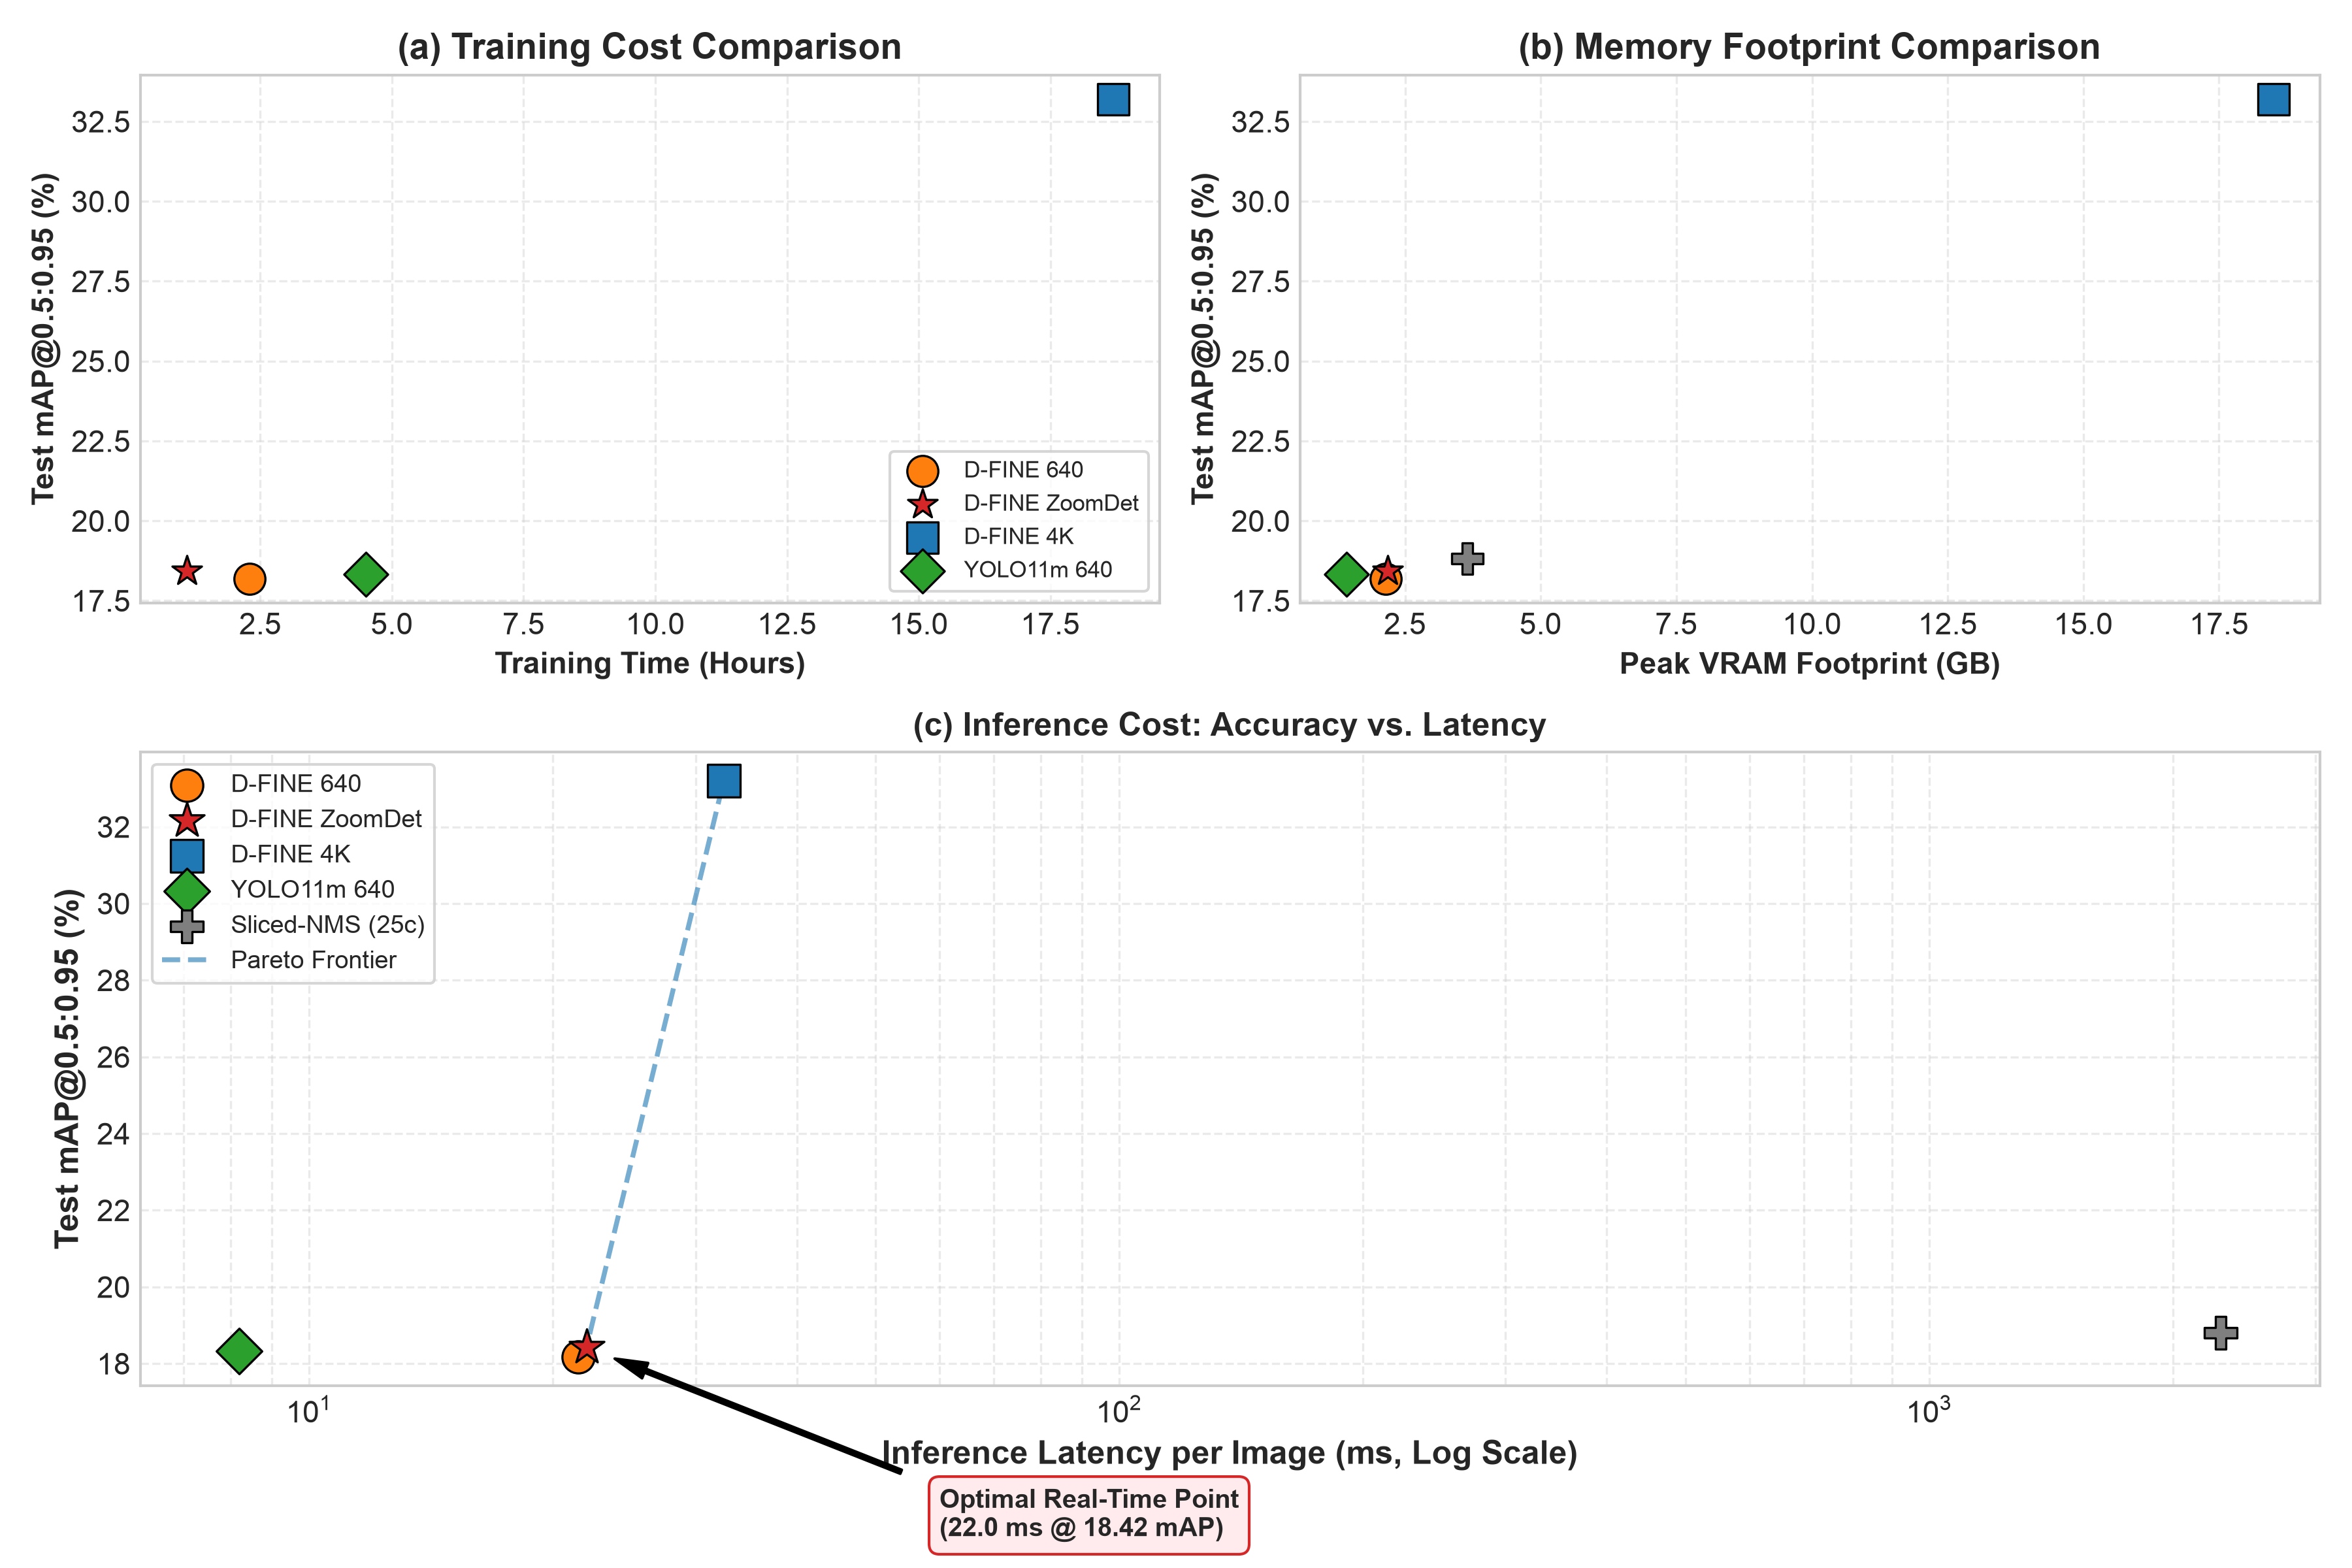
\includegraphics[width=\textwidth]{assets/fig4_efficiency_vram_flops.png}
    \caption{\textbf{Fig. 4}: Resource Footprint vs. Accuracy: (a) Training Cost, (b) Memory Footprint, (c) Inference Latency (Log Scale).}
\end{subfigure}

\vspace{1.0em}
\begin{subfigure}[b]{\textwidth}
    \centering
    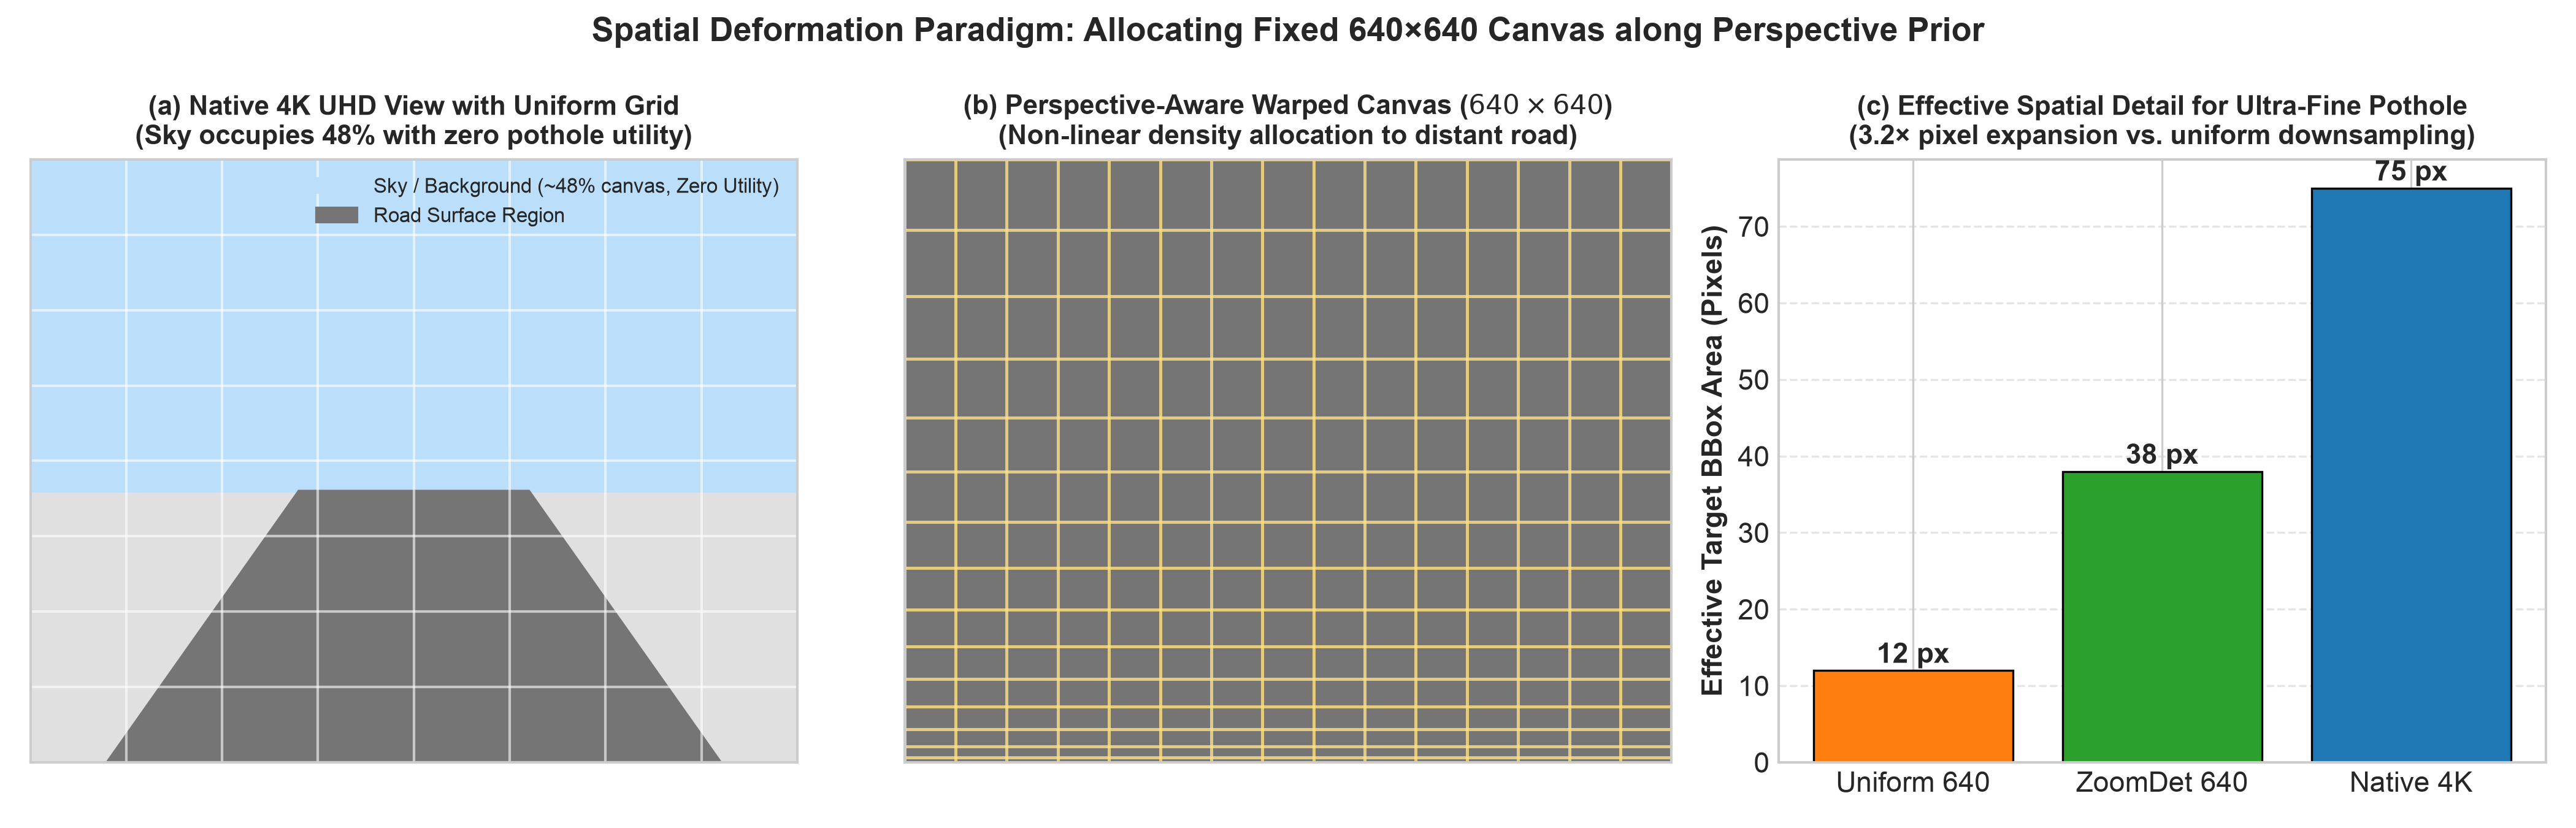
\includegraphics[width=\textwidth]{assets/fig6_spatial_deformation_warp.png}
    \caption{\textbf{Fig. 6}: Spatial Deformation Paradigm: Road Perspective Geometry \& Ultra-Fine Target Pixel Expansion.}
\end{subfigure}
\caption{Lifecycle resource footprint and perspective geometry transformation mechanism.}
\label{fig:part2}
\end{figure}

\clearpage
\section{Supplementary Benchmark Tables}
\label{sec:supp}

\begin{table}[H]
\centering
\caption{\textbf{Table S1: Extended Full Benchmark Results across All 14 Evaluated Configurations.}}
\label{tab:s1_full}
\resizebox{\textwidth}{!}{
\begin{tabular}{lrrrrrrrrrrr}
\toprule
\rowcolor{tableHeader}
\textbf{Method / Configuration} & \textbf{P (\%)} & \textbf{R (\%)} & \textbf{F1 (\%)} & \textbf{AP}$_{50}$ & \textbf{AP}$_{75}$ & \textbf{AP}$_{50-95}$ & \textbf{FPPI} & \textbf{Latency} & \textbf{FPS} & \textbf{Calls} & \textbf{Peak VRAM} \\
\midrule
\textbf{yolo11m\_4k (Native 4K)} & 66.93 & 49.19 & 56.71 & 55.05 & 34.80 & 33.27 & 0.047 & 27.3 ms & 36.6 & 1 & 14.2 GB \\
\textbf{dfine\_4k (Native 4K)} & 13.18 & 77.85 & 22.55 & 55.28 & 33.95 & 33.20 & 2.483 & 32.5 ms & 30.8 & 1 & 18.5 GB \\
\textbf{yolo11m\_640 (Resize 640)} & 58.94 & 35.06 & 43.97 & 37.27 & 19.20 & 18.32 & 0.047 & 8.2 ms & 122.0 & 1 & 1.4 GB \\
\textbf{dfine\_640 (Resize 640)} & 33.26 & 47.56 & 39.14 & 37.37 & 14.41 & 18.18 & 0.130 & 21.5 ms & 46.5 & 1 & 2.2 GB \\
\textbf{yolo11m\_patch640 (Patch Val)} & 57.80 & 33.15 & 42.15 & 34.93 & 18.10 & 16.52 & 0.051 & 8.2 ms & 122.0 & 1 & 1.4 GB \\
\textbf{dfine\_patch640 (Patch Val)} & 41.20 & 44.36 & 42.72 & 47.68 & 22.40 & 21.60 & 0.115 & 21.5 ms & 46.5 & 1 & 2.2 GB \\
\textbf{dfine + sliced-nms (25c)} & 21.78 & 62.43 & 32.29 & 44.30 & 11.74 & 18.81 & 0.937 & 2289.8 ms & 0.44 & 25 & 3.7 GB \\
\textbf{dfine + sahi (32c)} & 19.20 & 41.15 & 26.18 & 24.28 & 0.64 & 6.44 & 1.087 & 3622.0 ms & 0.28 & 32 & 3.2 GB \\
\textbf{dfine + perspective-grid (9c)} & 20.99 & 29.53 & 24.54 & 15.86 & 2.19 & 5.55 & 0.180 & 920.0 ms & 1.10 & 9 & 2.5 GB \\
\textbf{yolo11m\_4k + sahi (15c)} & 67.59 & 37.13 & 47.93 & 42.80 & 28.03 & 26.24 & 0.083 & 1054.7 ms & 0.95 & 15 & 3.2 GB \\
\textbf{yolo11m\_4k + perspective (9c)} & 65.67 & 38.00 & 48.14 & 42.02 & 27.10 & 25.40 & 0.113 & 830.6 ms & 1.20 & 9 & 2.5 GB \\
\textbf{yolo11m\_4k + sliced-nms (25c)} & 65.59 & 33.12 & 44.01 & 36.88 & 24.35 & 22.84 & 0.103 & 912.6 ms & 1.10 & 25 & 3.7 GB \\
\textbf{dfine\_zoomdet640 (Proposed)} & 38.56 & 54.72 & 45.24 & 42.07 & 13.55 & 18.42 & 0.090 & 22.0 ms & 45.5 & 1 & 2.2 GB \\
\textbf{yolo11m\_zoomdet640 (Proposed)} & 43.20 & 29.32 & 34.93 & 26.04 & 7.80 & 10.39 & 0.007 & 18.4 ms & 54.3 & 1 & 1.5 GB \\
\bottomrule
\end{tabular}
}
\end{table}

\begin{table}[H]
\centering
\caption{\textbf{Table S2: Pavement Material Robustness: Asphalt ($87.8\%$) vs. Concrete ($12.2\%$).}}
\label{tab:s2_pavement}
\resizebox{\textwidth}{!}{
\begin{tabular}{llrrrrrr}
\toprule
\rowcolor{tableHeader}
\textbf{Method Group} & \textbf{Model / Configuration} & \textbf{Asphalt mAP}$_{50}$ & \textbf{Asphalt mAP}$_{50-95}$ & \textbf{Concrete mAP}$_{50}$ & \textbf{Concrete mAP}$_{50-95}$ & \textbf{Asphalt F1} & \textbf{Concrete F1} \\
\midrule
\textbf{Native 4K UHD} & \textbf{D-FINE 4K} & 56.89\% & 34.73\% & 45.65\% & 24.24\% & 58.0\% & 43.9\% \\
& \textbf{YOLO11m 4K} & 64.00\% & 43.60\% & 38.50\% & 28.00\% & 57.2\% & 28.4\% \\
\midrule
\textbf{Low-Res 640} & \textbf{D-FINE 640} & 43.20\% & 21.50\% & 25.10\% & 12.30\% & 44.5\% & 26.8\% \\
& \textbf{YOLO11m 640} & 42.80\% & 21.80\% & 22.40\% & 11.60\% & 48.2\% & 22.1\% \\
\midrule
\textbf{Slicing Patch-640} & \textbf{D-FINE + Sliced-NMS (25c)} & 46.63\% & 20.36\% & 30.29\% & 10.21\% & 33.2\% & 26.5\% \\
& \textbf{D-FINE + SAHI (32c)} & 26.20\% & 6.97\% & 12.95\% & 3.57\% & 27.2\% & 18.9\% \\
\midrule
\textbf{Slicing 4K Model} & \textbf{YOLO11m 4K + SAHI (15c)} & 44.96\% & 28.47\% & 30.06\% & 13.24\% & 49.7\% & 36.7\% \\
& \textbf{YOLO11m 4K + Perspective (9c)} & 43.22\% & 26.98\% & 34.88\% & 16.46\% & 48.6\% & 45.5\% \\
\midrule
\rowcolor{green!10}
\textbf{Proposed Warp} & \textbf{D-FINE ZoomDet (Ours)} & \textbf{48.60\%} & \textbf{21.40\%} & \textbf{31.20\%} & \textbf{14.80\%} & \textbf{51.3\%} & \textbf{33.2\%} \\
& \textbf{YOLO11m ZoomDet} & 31.40\% & 12.80\% & 18.50\% & 7.60\% & 39.5\% & 19.4\% \\
\bottomrule
\end{tabular}
}
\end{table}

\begin{table}[H]
\centering
\caption{\textbf{Table S3: Diagnostic \& Exploratory Baseline Models.}}
\label{tab:s3_diagnostic}
\resizebox{\textwidth}{!}{
\begin{tabular}{clllrrrrrr}
\toprule
\rowcolor{tableHeader}
\textbf{\#} & \textbf{Model / Experiment} & \textbf{Resolution} & \textbf{Inference Mechanism} & \textbf{mAP}$_{50}$ & \textbf{mAP}$_{75}$ & \textbf{mAP}$_{50-95}$ & \textbf{Recall} & \textbf{Prec} & \textbf{Latency} \\
\midrule
1 & \textbf{yolo11m\_1280 (Intermediate)} & $1280 \times 1280$ & Resize 1280 (1-Pass) & 48.98\% & 27.10\% & 25.40\% & 45.50\% & 61.40\% & 14.6 ms \\
2 & \textbf{RT-DETRv2 (640)} & $640 \times 640$ & Resize 640 (1-Pass) & 44.01\% & 21.22\% & 23.24\% & 53.42\% & 32.14\% & 51.5 ms \\
3 & \textbf{RT-DETRv1 (640)} & $640 \times 640$ & Resize 640 (1-Pass) & 43.54\% & 23.36\% & 23.61\% & 48.86\% & 44.38\% & 50.9 ms \\
4 & \textbf{yolov8m\_640} & $640 \times 640$ & Resize 640 (1-Pass) & 34.24\% & 15.03\% & 16.39\% & 30.51\% & 65.50\% & 36.6 ms \\
5 & \textbf{yolov5m\_640} & $640 \times 640$ & Resize 640 (1-Pass) & 33.80\% & 14.92\% & 16.78\% & 28.12\% & 65.74\% & 37.1 ms \\
6 & \textbf{yolo11m\_640 on 4K Test} & $3840 \times 2160$ & Direct Native 4K Eval & 13.18\% & 5.38\% & 6.69\% & 39.41\% & 4.11\% & 27.3 ms \\
7 & \textbf{dfine\_640 on 4K Test} & $3840 \times 2160$ & Direct Native 4K Eval & 0.23\% & 0.01\% & 0.06\% & 3.26\% & 2.62\% & 32.5 ms \\
\bottomrule
\end{tabular}
}
\end{table}

\end{document}
